\documentclass{standalone}
\usepackage{tikz}

\newcounter{node}

\begin{document}
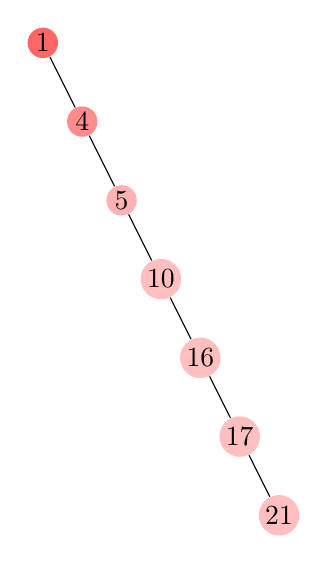
\begin{tikzpicture}
  [level distance=10mm,
    every node/.style={fill=red!60,circle,inner sep=1pt},
    level 1/.style={sibling distance=10mm,nodes={fill=red!45}},
    level 2/.style={sibling distance=10mm,nodes={fill=red!30}},
  level 3/.style={sibling distance=10mm,nodes={fill=red!25}},
]
  \node {1}
  child[missing] 
  child {node {4}
    child[missing]
    child {node {5}
       child[missing]
       child{node {10}
         child[missing]
         child{node {16}
            child[missing]
            child{node {17}
              child[missing]
              child{node {21}}
            }
         }
       }
    }
  };
\end{tikzpicture}
\end{document}





